\documentclass[14pt,aspectratio=169]{beamer}

\usepackage{pgfpages}
\usepackage{fancyvrb}
\usepackage{pgfplots}

\usepackage{minted}
\usemintedstyle{tango}

\usepackage{amsfonts}

\usepackage{moresize}
\usepackage{anyfontsize}

\usepackage{tikz}
\usetikzlibrary{arrows,shapes}
\usetikzlibrary{arrows.meta}

\tikzstyle{process}=[rectangle, draw, thick, text width=5em, text centered, minimum height=2.5em, fill=gray!40]
\tikzstyle{entity}=[rounded rectangle, draw, thick, text width=5em, text centered, minimum height=1.5em, fill=gray!40]

\usetheme{auriga}
\usecolortheme{auriga}

\setbeamercolor{background canvas}{bg=lightgray}

% define some colors for a consistent theme across slides
\definecolor{red}{RGB}{181, 23, 0}
\definecolor{blue}{RGB}{0, 118, 186}
\definecolor{gray}{RGB}{146, 146, 146}

\title{Discrete Structures: \\ Debugging Functions Implemented in Python}

\author{{\bf Gregory M. Kapfhammer}}

\institute[shortinst]{{\bf Department of Computer Science, Allegheny College}}

\begin{document}

{
  \setbeamercolor{page number in head/foot}{fg=background canvas.bg}
  \begin{frame}
    \titlepage
  \end{frame}
}

%% Slide
%
\begin{frame}{Technical Question}
  %
  \begin{center}
    %
    {\large How do I use debugging statements to better understand the behavior
      of functions that use iteration and recursion to perform mathematical
      operations such as computing the factorial sequence, the square of a number,
    and the mean and median of a sequence of numbers?}
    %
  \end{center}
  %
  \vspace{1ex}
  %
  \begin{center}
    %
    \small Let's learn how to use Python {\tt print} statements to debug
    functions that perform mathematical and statistical computations!
    %
  \end{center}
  %
\end{frame}

% Slide
%
\begin{frame}{Debugging Python Functions}
  %
  \begin{itemize}
    %
    \item Intuitively read the functions to grasp their behavior
      %
      \vspace*{-.15in}
      %
    \item Key components of the Python functions
      %
      \begin{itemize}
        %
        \item Definition of the function
          %
        \item Parameter(s) that serve as the input
          %
        \item Body that performs a computation
          %
        \item Function return value(s) that produce output
          %
        \item Invocation of the function
          %
        \item Collecting the output of the function
          %
        \item Test case(s) for the function
          %
      \end{itemize}
      %
      \vspace*{-.2in}
      %
    \item Learn how {\tt print} statements can create debugging output,
      helping to understand a function's behavior
      %
  \end{itemize}
  %
\end{frame}

% Slide
%
\begin{frame}[fragile]
  \frametitle{Understanding the {\tt range} Function in Python}
  \normalsize
  % \hspace*{-.15in}
  \begin{minipage}{6in}
    \vspace*{.25in}
    \begin{minted}[mathescape, numbersep=5pt, fontsize=\large]{python}
for i in range(20):
    print("Value of i: " + str(i))
    \end{minted}
  \end{minipage}
  \vspace*{.25in}
  \begin{center}
    %
    \normalsize \noindent The {\tt range} function returns the values from 0 to 19 \\
    \normalsize \noindent The {\tt for} loop displays the value of {\tt i} from 0 to 19 \\
    \normalsize \noindent The {\tt str} function converts an integer to a string \\
    \normalsize \noindent The {\tt print} statement aids understanding of
    loop behavior \\
    %
  \end{center}
  %
\end{frame}

% Slide
%
\begin{frame}[fragile]
  \frametitle{Output of Program Using the {\tt range} Function}
  \normalsize
  % \hspace*{-.15in}
  \begin{minipage}{6in}
    \vspace*{.25in}
    \begin{minted}[mathescape, numbersep=5pt, fontsize=\small]{text}
Value of i: 0
Value of i: 1
Value of i: 2
Value of i: 3
Value of i: 4
Value of i: 5
Value of i: 6
Value of i: 7
Value of i: 8
Value of i: 9
    \end{minted}
  \end{minipage}
  \vspace*{.05in}
  \begin{center}
    %
    \normalsize \noindent The {\tt print} statements sheds light on the
  function's behavior!\\
    %
  \end{center}
  %
\end{frame}

% Slide
%
\begin{frame}[fragile]
  \frametitle{Output of Program Using the {\tt range} Function}
  \normalsize
  % \hspace*{-.15in}
  \begin{minipage}{6in}
    \vspace*{.25in}
    \begin{minted}[mathescape, numbersep=5pt, fontsize=\small]{text}
Value of i: 10
Value of i: 11
Value of i: 12
Value of i: 13
Value of i: 14
Value of i: 15
Value of i: 16
Value of i: 17
Value of i: 18
Value of i: 19
    \end{minted}
  \end{minipage}
  \vspace*{.05in}
  \begin{center}
    %
    \normalsize \noindent How many times did the {\tt for} loop run? How did
    you know?\\
    %
  \end{center}
  %
\end{frame}

% Slide
%
\begin{frame}[fragile]
  \frametitle{Using {\tt for} Loops in Python Programs}
  \normalsize
  \hspace*{-.65in}
  \begin{minipage}{6in}
    \vspace*{.25in}
    \begin{minted}[mathescape, numbersep=5pt, fontsize=\large]{python}
    for i in range(20):
        print("2 to the " + str(i)
              + " power is " + str(2**i))
    \end{minted}
  \end{minipage}
  \vspace*{.25in}
  \begin{center}
    %
    \normalsize \noindent The {\tt for} loop displays the powers of 2 from 0 to 19 \\
    \normalsize \noindent The {\tt range} function returns the values from 0 to 19 \\
    \normalsize \noindent The {\tt 2**i} performs the computation of $2^i$ \\
    \normalsize \noindent The {\tt str} function converts an integer to a string \\
    %
  \end{center}
  %
\end{frame}

% Slide
%
\begin{frame}[fragile]
  \frametitle{Output of a Python Program Using Iteration}
  \normalsize
  % \hspace*{-.35in}
  \begin{minipage}{6in}
    \vspace*{.25in}
    \begin{minted}[mathescape, numbersep=5pt, fontsize=\small]{text}
2 to the 0 power is 1
2 to the 1 power is 2
2 to the 2 power is 4
2 to the 3 power is 8
2 to the 4 power is 16
2 to the 5 power is 32
2 to the 6 power is 64
2 to the 7 power is 128
2 to the 8 power is 256
2 to the 9 power is 512
    \end{minted}
  \end{minipage}
  \vspace*{.05in}
  \begin{center}
    %
    \normalsize \noindent Function output helps to understand the {\tt for} loop's behavior!\\
    %
  \end{center}
  %
\end{frame}

% Slide
%
\begin{frame}[fragile]
  \frametitle{Output of a Python Program Using Iteration}
  \normalsize
  \hspace*{-.35in}
  \begin{minipage}{6in}
    \vspace*{.25in}
    \begin{minted}[mathescape, numbersep=5pt, fontsize=\small]{text}
    2 to the 10 power is 1024
    2 to the 11 power is 2048
    2 to the 12 power is 4096
    2 to the 13 power is 8192
    2 to the 14 power is 16384
    2 to the 15 power is 32768
    2 to the 16 power is 65536
    2 to the 17 power is 131072
    2 to the 18 power is 262144
    2 to the 19 power is 524288
    \end{minted}
  \end{minipage}
  \vspace*{.05in}
  \begin{center}
    %
    \normalsize \noindent Any questions about the  {\tt for} loop's behavior?\\
    %
  \end{center}
  %
\end{frame}

% Slide
%
\begin{frame}[fragile]
  \frametitle{Using {\tt while} Loops in Python Programs}
  \normalsize
  \hspace*{-.65in}
  \begin{minipage}{6in}
    \vspace*{.25in}
    \begin{minted}[mathescape, numbersep=5pt, fontsize=\large]{python}
    i = 0
    while i < 20:
        print("2 to the " + str(i)
              + " power is " + str(2**i))
        i += 1
    \end{minted}
  \end{minipage}
  \vspace*{.1in}
  \begin{center}
    %
    \normalsize \noindent The purpose of {\tt i += 1} is to increment the loop counter\\
    \normalsize \noindent The {\tt print} statement is the same in {\tt for} and
    {\tt while }loops\\
    \normalsize \noindent Can you trace the execution of this iteration
    construct?\\
    %
  \end{center}
  %
\end{frame}

% Slide
%
\begin{frame}[fragile]
  \frametitle{Recursive Functions in Python Programs}
  \hspace*{-.8in}
  \begin{minipage}{6in}
    \begin{minted}[mathescape, numbersep=5pt, fontsize=\large]{python}
    def factorial(number: int):
        if number == 1:
            return 1
        return number * factorial(number - 1)

    num = 5
    print("The factorial of " + str(num) +
           " is " + str(factorial(num)))
    \end{minted}
  \end{minipage}
  \vspace*{.05in}
\end{frame}

% Slide
%
\begin{frame}{Recursive Computation of the Factorial Function}
  %
  \begin{itemize}
    %
    \item As an equation: $n! = n \times n-1 \times n-2 \times \ldots \times 1$
      %
      \vspace*{-.15in}
      %
    \item What are the parts of a recursive function in Python?
      %
      \begin{itemize}
        %
        \item Defined by cases using conditional logic
          %
        \item A function definition that calls itself
          %
        \item A recursive call that makes progress to a base case
          %
        \item A base case that stops the recursive function calls
          %
      \end{itemize}
      %
      \vspace*{-.2in}
      %
    \item Repeatedly perform an operation through function calls
      %
      \vspace*{-.2in}
      %
    \item Can you find all the components of this recursive function?
      %
      \vspace*{-.4in}
      %
    \item Can you explain how this recursive function behaves?
      %
  \end{itemize}
  %
\end{frame}

% Slide
%
\begin{frame}[fragile]
  \frametitle{Finding the Parts of a Recursive Function}
  \hspace*{-.8in}
  \begin{minipage}{6in}
    \begin{minted}[mathescape, numbersep=5pt, fontsize=\large]{python}
    def factorial(number: int):
        if number == 1:
            return 1
        return number * factorial(number - 1)

    num = 5
    print("The factorial of " + str(num) +
           " is " + str(factorial(num)))
    \end{minted}
  \end{minipage}
  \vspace*{.05in}
\end{frame}

% Slide
%
\begin{frame}[fragile]
  \frametitle{Output of a Python Program Using Recursion}
  \normalsize
  \begin{minipage}{6in}
    \vspace*{.25in}
    \begin{minted}[mathescape, numbersep=5pt, fontsize=\small]{text}
Current call factorial(5)
  ... Now calling factorial(4)
Current call factorial(4)
  ... Now calling factorial(3)
Current call factorial(3)
  ... Now calling factorial(2)
Current call factorial(2)
  ... Now calling factorial(1)
Current call factorial(1)
  ... Hit the base case!
The factorial of 5 is 120
    \end{minted}
  \end{minipage}
  \vspace*{.05in}
  \begin{center}
    %
    \normalsize \noindent The debugging output shows that the function calls
    itself!\\
    %
  \end{center}
  %
\end{frame}

% Slide
%
\begin{frame}[fragile]
  \frametitle{Creating Higher-Order Functions in Python}
  \hspace*{-.6in}
  \begin{minipage}{6in}
    \begin{minted}[mathescape, numbersep=5pt, fontsize=\large]{python}
    def square(number: int):
        return number * number

    def call_twice(f, number: int):
        return f(f(number))

    number = 5
    result = call_twice(square, number)
    \end{minted}
  \end{minipage}
  \vspace*{.05in}
\end{frame}

% Slide
%
\begin{frame}[fragile]
  \frametitle{Program Output with Higher-Order Functions}
  \normalsize
  \begin{minipage}{6in}
    \vspace*{.25in}
    \begin{minted}[mathescape, numbersep=5pt, fontsize=\small]{text}
Calling twice <function square at 0x7f36331d01f0> with
  starting number of 5
Called square(5)
  returning 25
Called square(25)
  returning 625

Calling the square twice with 5 is 625

Direct computation of twice square is 5 is 625
    \end{minted}
  \end{minipage}
  \vspace*{.05in}
  \begin{center}
    %
    \normalsize \noindent What is the meaning of the {\tt 0x7f36331d01f0}
    notation?\\
    %
  \end{center}
  %
\end{frame}

% Slide
%
\begin{frame}{Creating Functions for Statistical Analysis}
  %
  \begin{figure}
    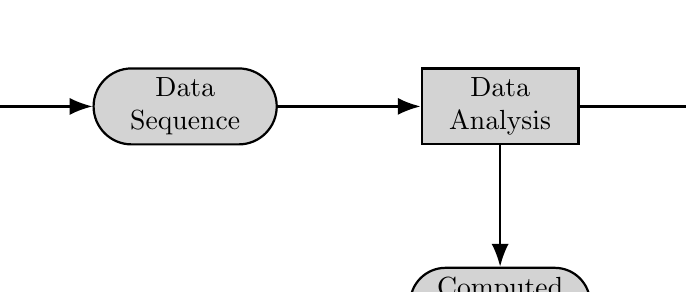
\begin{tikzpicture}[node distance=4cm, auto,>=latex', thick]
      %
      \path[use as bounding box] (2,1) rectangle (10,-2);
      %
      % Sensor* --> Data Sequence*
      %
      \path[->] node[process, font=\large] (sensor) {Sensor};
      \path[->] node[entity, right of=sensor, align=center] (values) {Data \\ Sequence};
      \path [draw, thick, -{>[scale=1.25]}, >=Latex] (sensor.east) -- (values.west);
      %
      % Data Sequence --> Data Analysis*
      %
      \path[->] node[process, right of=values, align=center] (analyze) {Data \\ Analysis};
      \path [draw, thick, -{>[scale=1.25]}, >=Latex] (values.east) -- (analyze.west);
      %
      % Data Analysis --> Computed Mean*
      %
      \path[->] node[entity, below of=analyze, align=center, yshift=1.5cm]
        (average) {Computed \\ Mean};
      \path [draw, thick, -{>[scale=1.25]}, >=Latex] (analyze.south) -- (average.north);
      %
      % Data Analysis --> Data Visualization*
      %
      \path[->] node[entity, right of=analyze, align=center] (graph) {Data \\ Graph};
      \path [draw, thick, -{>[scale=1.25]}, >=Latex] (analyze.east) -- (graph.west);
      %
    \end{tikzpicture}
    %
    \vspace*{.6in}
    \begin{center}
      %
      \normalsize
      %
      \noindent How do we compute the {\em mean} of a list of numbers? \\
      \noindent How do we compute summary statistics of a list of numbers? \\
      \noindent What type of function? Recursive? Iterative? Lambda?
      %
    \end{center}
    %
  \end{figure}
  %
\end{frame}

% Slide
%
\begin{frame}{Implementing and Debugging Python Functions}
  %
  \begin{itemize}
    %
    \item Use debugging statements to grasp a function's behavior!
      %
      \vspace*{-.15in}
      %
    \item Python functions to perform statistical analysis of data
      %
      \begin{itemize}
        %
        \item {\bf Q1}: How do you compute the median of a list of numbers?
          %
        \item {\bf Q2}: How do you compute the mode of a list of numbers?
          %
        \item {\bf Q3}: How do you compute a frequency table of a list of
          numbers?
          %
        \item {\bf Q4}: How do you compute the range of a list of numbers?
          %
        \item {\bf Q5}: How do you compute the variance and standard deviation?
          %
      \end{itemize}
      %
      \vspace*{-.2in}
      %
    \item Can you translate the mathematical descriptions of these summary
      statistics to Python programs? Can you ensure their correctness? Can you
      follow industry best practices?
      %
  \end{itemize}
  %
\end{frame}

\end{document}
